\section{Results}
\subsection{Toy Data Experiment}
\label{app_toy_data_gen}
The 2-D toy data (represented as $x=\{x_1, x_2\}$) is generated from a Markov model with 4 states (states 0, 1, 2, 3) with the means of the emission distributions located at $(0, -1), (8, -1), (13, 0)$ and $(24, 0)$. The variance in $x_1$ is 0.3 and variance in $x_2$ is 1 for each of the clusters. Each sequence is initialized at state 0 and either remains in the current state or transitions to the next adjacent state with equal probability. Once state 2 is reached, it immediately transitions to state 3 in the next time-step and stays there for the remaining time-steps with probability 1. We simulate 350 sequences, each of length $T=8$ from this model. A sequence is labeled as 1 if it enters the highlighted black box highlighted in figure \ref{fig:toy_pchmm} at any time-point. At each time-point and dimension, data is missing with a fixed probability ($\rho$). We vary $\rho$ on the right plot of figure \ref{fig:toy_pchmm} and report classification performance against several baselines. 

\textbf{Findings :}
We analyze a toy dataset of many sequences generated by an HMM with $K=4$ Gaussian clusters in a $D=2$ feature space. The 2D features are illustrated in Fig.~\ref{fig:toy_pchmm}:
Each sequence is labeled $y=1$ only if any timestep's feature $x_t$ enters the black square.
Fig.~\ref{fig:toy_pchmm} (left) shows that even at 40\% missingness (i.i.d. across features and timesteps) the PC-HMM with $K=6$ learns separate states that cover the black box and its complement, and thus are \emph{discriminative}.
In contrast, both mean-filling and forward-filling imputation destroy the separability of red and blue classes. 
In Fig.~\ref{fig:toy_pchmm} (right), at all missingness levels the PCHMM delivers better AUROC than alternatives, including an LSTM and the GRU-D. This dataset is class-balanced, thus AUROC is an appropriate metric. Later mortality prediction tasks are imbalanced, so we use area under the precision recall curve (AUPRC) instead.
All PC-HMM results, including ``with mean-filled/forward-filled'' baselines, assume diagonal covariances.

\setlength{\tabcolsep}{.1cm}
\begin{figure*}[!t]
\begin{tabular}{c c}
    \centering
% Suggestion 1: Always specify either height or weight
% Suggestion 2: Make sure the aspect ratio when exported matches the intended ratio in the paper here
    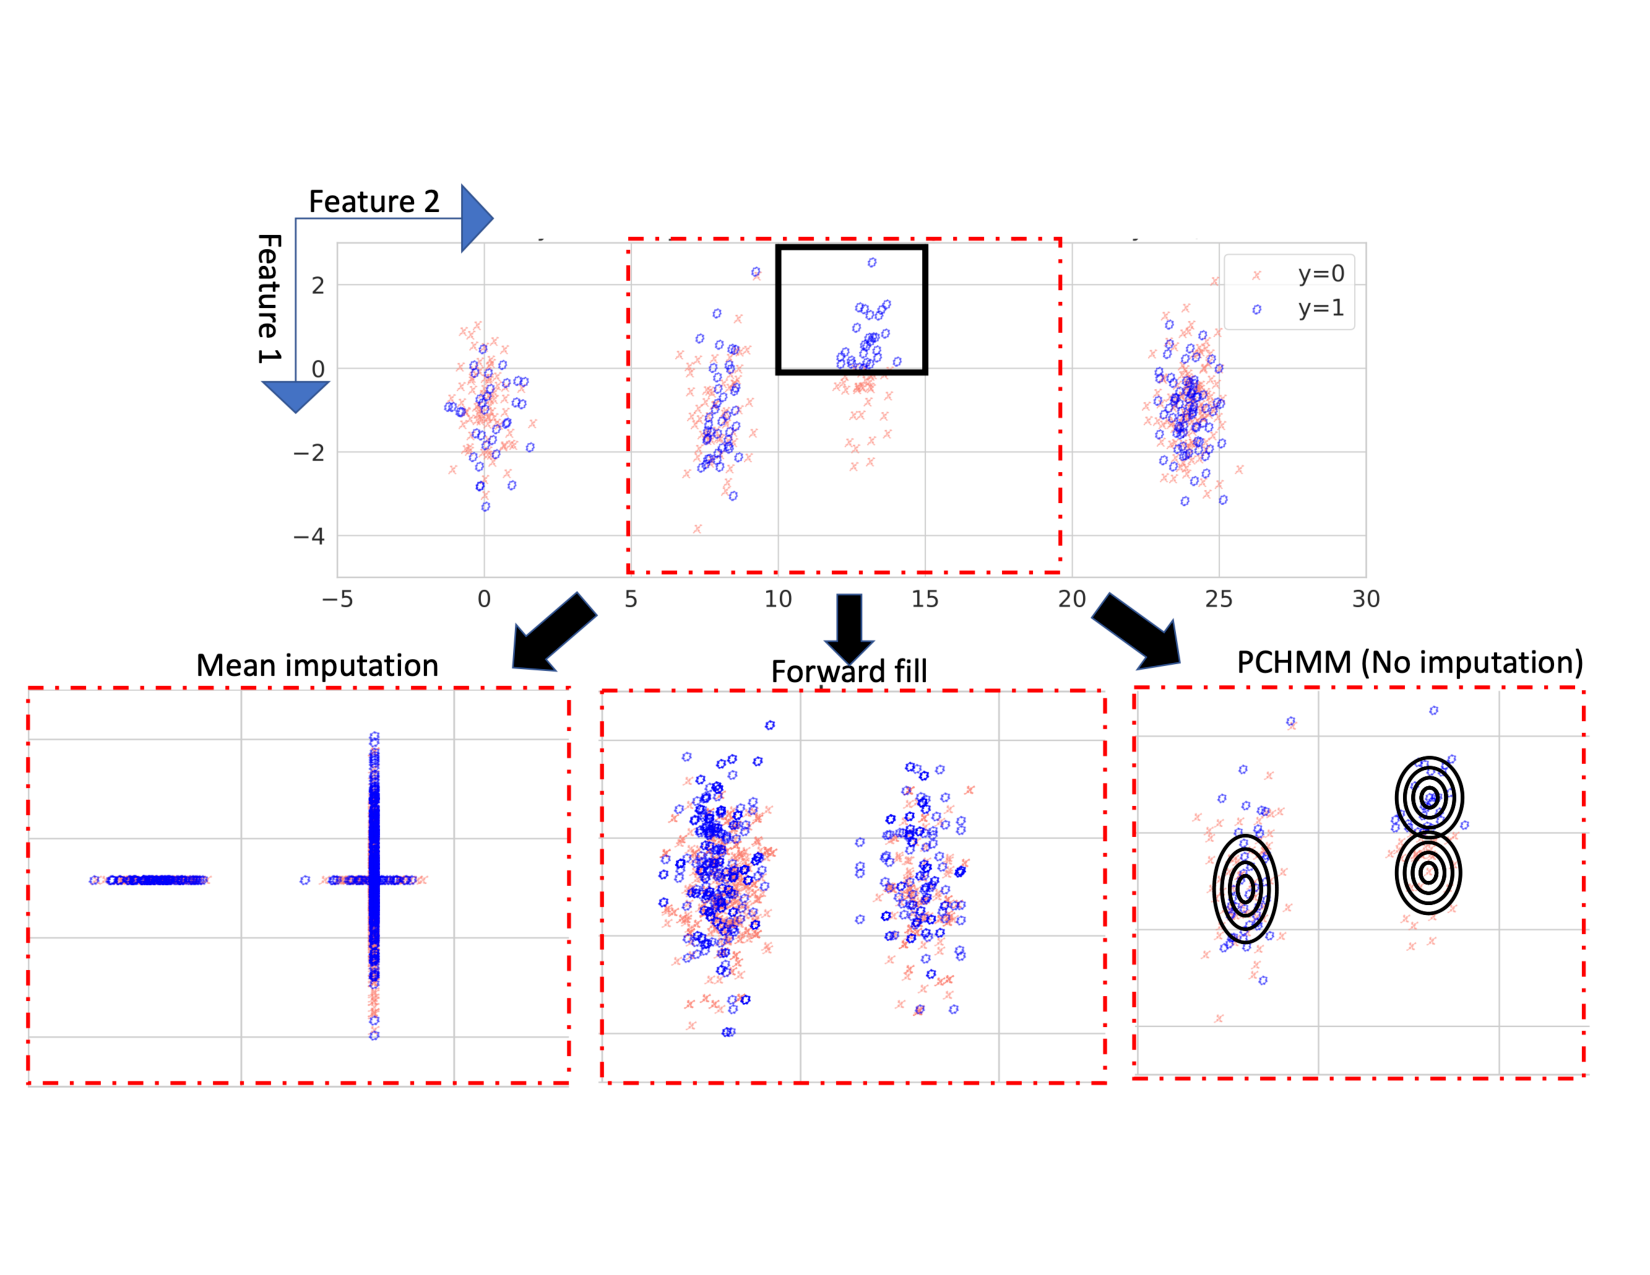
\includegraphics[width=0.57\textwidth]{content/chapters/semi_supervised_pchmm_missing_data/images/toy_data_fig.pdf}
    &
    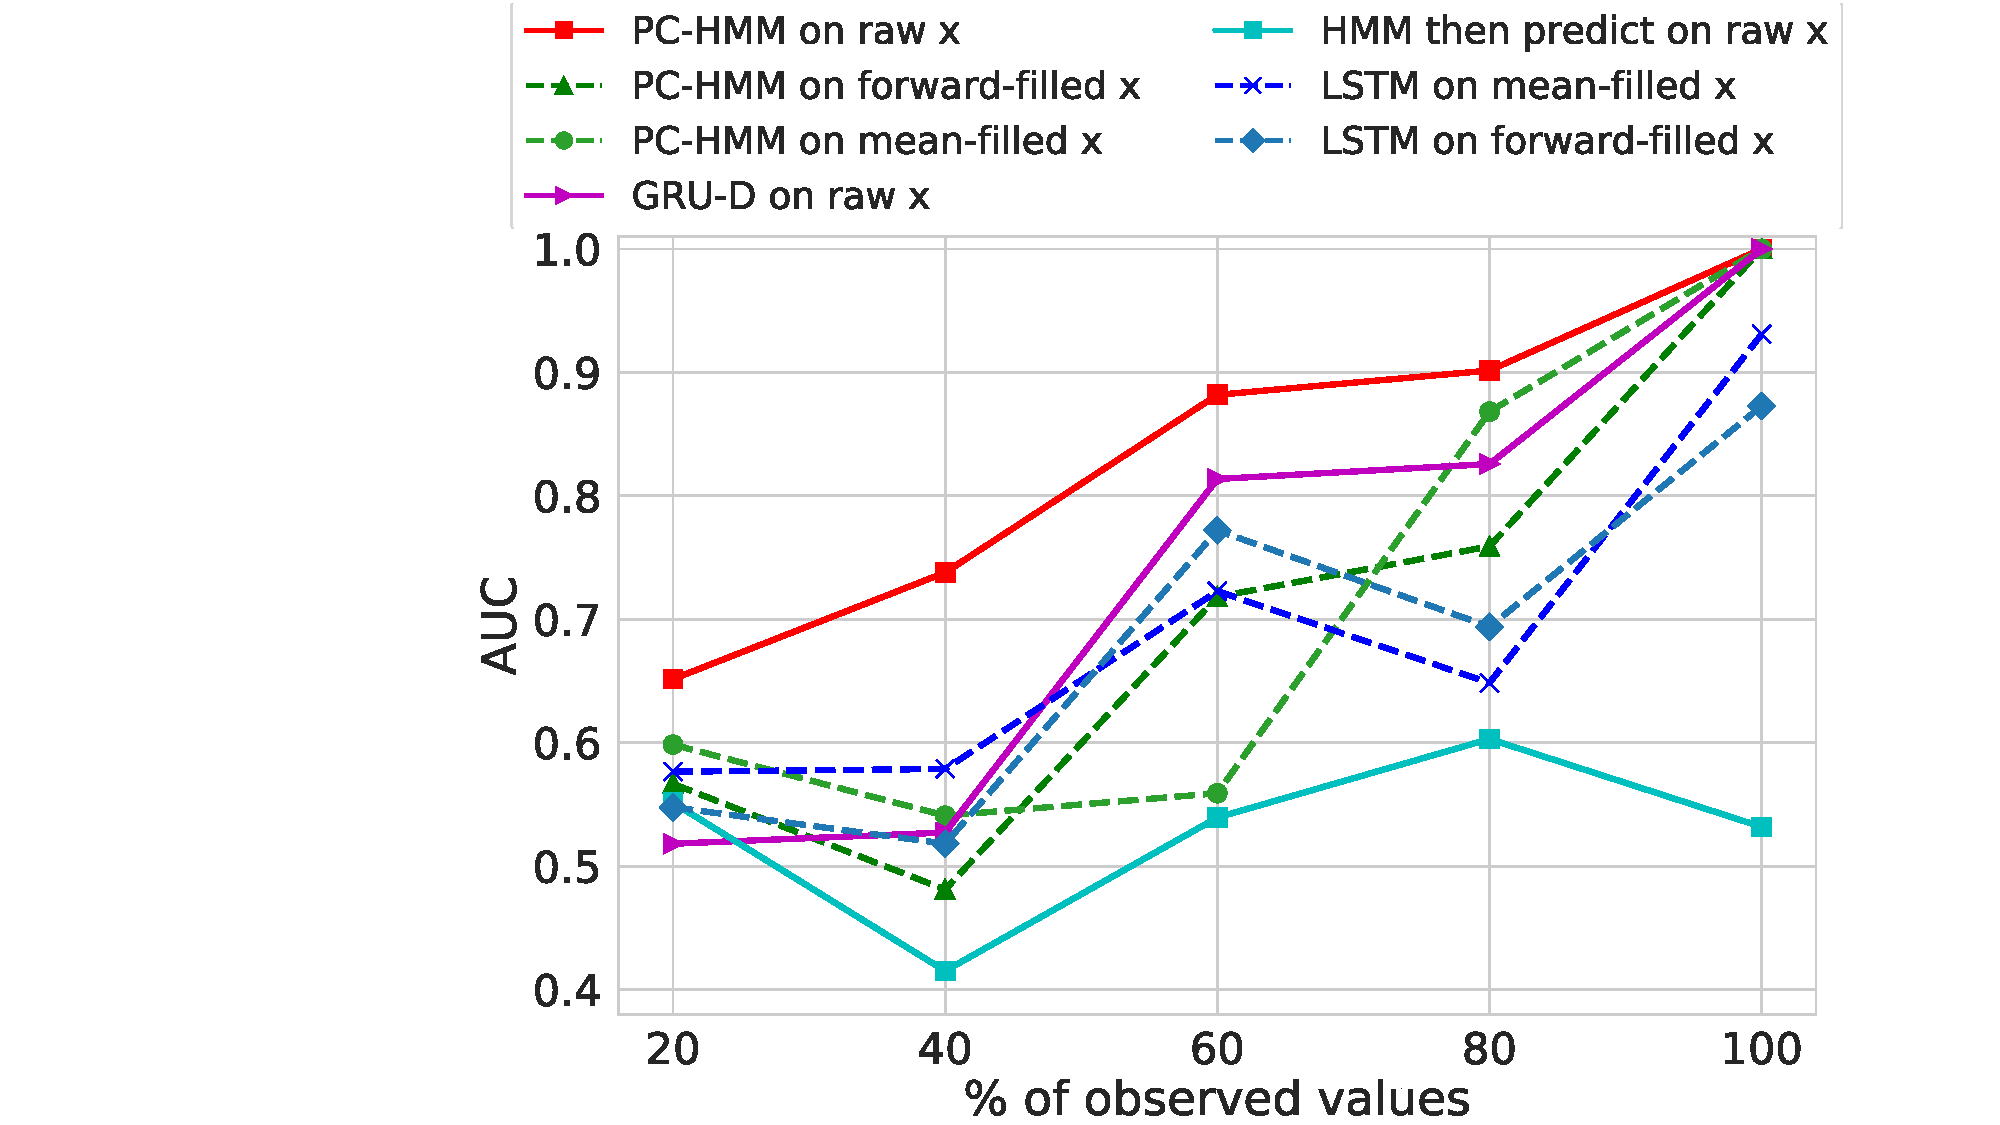
\includegraphics[width=0.43\textwidth]{content/chapters/semi_supervised_pchmm_missing_data/images/toy_data_perf_fig.pdf}
\end{tabular}
\caption[Demonstration of proposed PC-HMM on an “easy” binary classifier
task where naive imputation fails]{Demonstration of proposed PC-HMM on an ``easy'' binary classifier task where naive imputation fails.
\textbf{\emph{Top left:}} Visualization of all observed 2D features from 350 sequences (x-axis: feature 1 value, y-axis: feature 2), colored by labels and collapsed over time.
Each sequence ($T{=}8$) comes from a Markov model that generates features from the 4 clusters shown in this 2D feature space.
A sequence's class label depends on if \emph{any observation} lands in the black box (yes means $y=1$, no means $y=0$). 
Without missingness, the two classes are clearly separable: compare black box to region below it.
\textbf{\emph{Bottom left:}} We sample features as missing with 40\% probability i.i.d. across timesteps and features. We then apply mean-filling or forward-filling: each panel shows 2D values \emph{after} imputation.
Either strategy clearly destroys class separability. 
Our PC-HMM does not need imputation, and even at 40\% missingness can learn to separate the black box from the region below it with separate Gaussian emission densities (black elipsoids).
\textbf{\emph{Right:}} AUROC vs. percentage of feature values observed. Across every tested percentage, our PC-HMM with compact state space (only 6 states, 80 total parameters) can outperform GRU-D or LSTM models even with many more parameters. 
}%endcaption
\label{fig:toy_pchmm}
\end{figure*}

\subsection{Real Data Experiments}
Below, we define and motivate two concrete prediction tasks that we pursue in our experimental evaluations.
Both tasks assume access to the first full 24 hour period of observation in critical care, and predict a future outcome.
To avoid causal leakage and ensure predictions could be actionable, in all training and evaluation data we only examine patient stays that last at least 30 hours. This prevents the classifier from learning a shortcut signal that is already quite obvious to the care team (e.g. lots of palliative morphine before death).

\textbf{In-ICU Mortality.} 
Given a few dozen vital sign and lab measurements from the first 24 hours of a patient stay, we wish to predict whether that patient will later die in the ICU ($y=1$) or not ($y=0$). 
Classifiers that can effectively predict an increased risk of mortality several hours ahead could be useful as early warning systems \citep{purushothamBenchmarkingDeepLearning2018, harutyunyanMultitaskLearningBenchmarking2019a, gao2020machine, rajkomar2018scalable}. 
Several of these works have pursued classifiers for in-ICU mortality. Our work is differentiated because our probabilistic approach does not rely on any form of imputation or iterative refinement of missing values, which are common in health record datasets. We further evaluate performance where labels are limited. While we acknowledge that a clinical outcome like in-ICU mortality outcome would rarely be missing, our goal is to use this outcome as a proxy to demonstrate the utility of our model for disease outcomes that require significant clinical expertise to annotate. To assess in-ICU mortality, we focus on area under the precision-recall curve (AUPRC) because it accounts for several limiting factors in clinical EHR prediction such as severe class imbalance, need for high performance on the positive class at low false alarm rates.

\subsection{Data}
\textbf{MIMIC-IV} We first study data from MIMIC-IV \cite{johnson2020mimic} to predict length of stay for 52,354 de-identified ICU  patient-stays from one hospital. We pre-process the dataset to contain 39 time varying measurements of labs and vitals and 2 demographics (see tables \ref{tab:mimic_features} and \ref{tab:eicu_features} for full feature list and missing data information). We selected these labs and vitals after reviewing existing literature pursuing prediction tasks with clinical time-series \citep{harutyunyanMultitaskLearningBenchmarking2019a, purushothamBenchmarkingDeepLearning2018}. Each time varying measurement is transformed into hourly buckets by taking the closest to the nearest earlier hour. If no data existed within an hourly bucket, we leave it as missing. We remove patient stays less than 30 hours to avoid label leakage. Additionally, we ensure that the subjects are split into train/valid and test based on patient-IDs.
\begin{table*}[h!]
  \centering
  \caption{MIMIC-IV features}
  \label{app:table_mimic_features}
  \begin{tabular}{lcccc}
    \toprule
    & 10\% & median & 90\% & missing\_rate \\
    \midrule
    Heart Rate	& 63.00 & 83.00 & 109.00 & 0.00 \\
    Respiratory Rate	& 13.00 & 18.00 & 26.00 & 0.00 \\
    O2 saturation pulseoxymetry	& 93.00 & 97.00 & 100.00 & 0.00 \\
    Non Invasive Blood Pressure systolic	& 93.00 & 116.00 & 148.00 & 0.08 \\
    Non Invasive Blood Pressure diastolic	& 47.00 & 63.00 & 85.00 & 0.08 \\
    Temperature Fahrenheit	& 36.22 & 36.83 & 37.61 & 0.07 \\
    Height (cm)	& 155.00 & 170.00 & 183.00 & 0.98 \\
    Respiratory Rate (Total)	& 14.00 & 18.00 & 27.00 & 0.62 \\
    Potassium (serum)	& 3.40 & 4.10 & 5.10 & 0.04 \\
    Sodium (serum)	& 132.00 & 138.00 & 144.00 & 0.04 \\
    Chloride (serum)	& 96.00 & 104.00 & 112.00 & 0.04 \\
    Hematocrit (serum)	& 23.60 & 30.30 & 38.90 & 0.05 \\
    Hemoglobin	& 7.70 & 10.10 & 13.10 & 0.05 \\
    Creatinine (serum)	& 0.60 & 1.00 & 3.10 & 0.04 \\
    Glucose (serum)	& 88.00 & 126.00 & 222.00 & 0.05 \\
    Magnesium	& 1.60 & 2.00 & 2.60 & 0.08 \\
    Phosphorous	& 2.20 & 3.50 & 5.50 & 0.11 \\
    Platelet Count	& 79.00 & 175.00 & 322.00 & 0.05 \\
    Glucose (whole blood)	& 97.00 & 136.00 & 200.00 & 0.77 \\
    Daily Weight	& 58.40 & 82.30 & 114.00 & 0.66 \\
    Absolute Neutrophil Count	& 4.55 & 9.30 & 20.54 & 1.00 \\
    Prothrombin time	& 11.60 & 14.20 & 23.60 & 0.21 \\
    Fibrinogen	& 127.00 & 216.00 & 462.00 & 0.80 \\
   PH (Arterial) & 7.25 & 7.37 & 7.46 & 0.60 \\
    PH (Venous) & 7.23 & 7.36 & 7.45 & 0.78 \\
    HCO3 (serum) & 17.00 & 23.00 & 28.00 & 0.05 \\
    Arterial O2 pressure & 75.00 & 132.00 & 334.00 & 0.60 \\
    Arterial CO2 Pressure & 31.00 & 40.00 & 52.00 & 0.60 \\
    Lactic Acid & 1.00 & 2.00 & 5.60 & 0.47 \\
    Albumin & 2.20 & 3.10 & 3.90 & 0.75 \\
    Calcium non-ionized & 7.30 & 8.30 & 9.30 & 0.12 \\
    C Reactive Protein (CRP) & 2.00 & 40.70 & 213.40 & 0.98 \\
    ALT & 11.00 & 33.00 & 395.00 & 0.59 \\
    AST & 17.00 & 48.00 & 568.00 & 0.59 \\
    Direct Bilirubin & 0.30 & 1.60 & 7.80 & 0.97 \\
    Total Bilirubin & 0.30 & 0.80 & 5.10 & 0.60 \\
    Troponin-T & 0.01 & 0.07 & 1.60 & 0.71 \\
    Venous CO2 Pressure & 30.00 & 42.00 & 63.00 & 0.82 \\
    Age & 40.00 & 65.00 & 84.00 & 0.00 \\
    is\_gender\_male & 0.00 & 1.00 & 1.00 & 0.00 \\
    is\_gender\_unknown & 0.00 & 0.00 & 0.00 & 0.00 \\
    \bottomrule
\end{tabular}
\end{table*}

\begin{table}[H]
\centering
\caption{MIMIC-IV Dataset Split and Statistics}
\label{tab:mimic-dataset-split}
\begin{tabular}{|l|l|c|c|c|c|c|c|}
\hline
\multirow{2}{*}{Dataset} & \multirow{2}{*}{Split} & \multirow{2}{*}{Stays} & \multirow{2}{*}{Patients} & \multicolumn{3}{c|}{Fraction of Stays} & \multirow{2}{*}{In-ICU mortality}\\ \cline{5-7}
 &  &  &  & LOS $\geq$ 3 days & LOS $\geq$ 7 days & LOS $\geq$ 11 days & \\ \hline
\multirow{3}{*}{MIMIC-IV} & Train & 33,506 & 27,084 & 0.46 & 0.16 & 0.08 &0.08 \\ \cline{2-8}
 & Valid & 8,377 & 7,821 & 0.46 & 0.16 & 0.08 & 0.08\\ \cline{2-8}
 & Test & 10,471 & 9,673 & 0.47 & 0.17 & 0.08 & 0.08 \\ \hline
\end{tabular}
\end{table}

\textbf{eICU} We also study the eICU dataset \cite{eICU} (details in section \ref{eicu_dataset_description}), containing 111,879 de-identified ICU patient-stays. We follow the same pre-processing steps as MIMIC-IV to aggregate measurements into hourly buckets, and split the data into train/valid and test, and remove stays less than 30 hours. We pre-process the dataset to contain 39 time varying measurements of labs and vitals and 2 demographics. 
\label{eicu_dataset_description}
\begin{table*}[h!]
\centering
\caption{eICU features}
\label{app:table_eicu_features}
\begin{tabular}{lcccc}
    \toprule
    Lab Test & 10\% & Median & 90\% & Missing Rate \\
    \midrule
    temperature & 35.80 & 37.18 & 38.21 & 0.91 \\
    sa02 & 93.25 & 97.17 & 100.00 & 0.04 \\
    heartrate & 62.42 & 82.83 & 108.92 & 0.03 \\
    respiration & 13.42 & 18.67 & 26.67 & 0.10 \\
    systemlicsystolic & 94.50 & 118.25 & 150.40 & 0.78 \\
    systemlicdiastolic & 44.25 & 57.45 & 75.42 & 0.78 \\
    ALT (SGPT) & 12.00 & 29.00 & 178.00 & 0.56 \\
    AST (SGOT) & 14.00 & 35.00 & 268.00 & 0.55 \\
    BUN & 9.00 & 21.00 & 59.00 & 0.07 \\
    Hct & 23.40 & 31.30 & 40.90 & 0.08 \\
    Hgb & 7.70 & 10.30 & 13.60 & 0.09 \\
    MCH & 26.70 & 30.00 & 32.70 & 0.16 \\
    PT & 11.60 & 15.60 & 27.00 & 0.61 \\
    RBC & 2.63 & 3.57 & 4.62 & 0.10 \\
    WBC x 1000 & 5.70 & 11.00 & 20.90 & 0.09 \\
    albumin & 1.90 & 2.80 & 3.70 & 0.52 \\
    anion gap & 6.00 & 11.00 & 18.00 & 0.26 \\
    calcium & 7.20 & 8.20 & 9.20 & 0.09 \\
    chloride & 96.00 & 105.00 & 113.00 & 0.07 \\
    creatinine & 0.59 & 1.08 & 3.38 & 0.06 \\
    glucose & 90.00 & 132.00 & 235.00 & 0.07 \\
    platelets x 1000 & 87.00 & 181.00 & 313.00 & 0.10 \\
    potassium & 3.30 & 4.00 & 5.00 & 0.05 \\
    sodium & 132.00 & 139.00 & 145.00 & 0.06 \\
    total bilirubin & 0.30 & 0.70 & 2.50 & 0.56 \\
    total protein & 4.60 & 5.80 & 7.00 & 0.55 \\
    uric acid & 2.70 & 6.10 & 11.90 & 0.98 \\
    magnesium & 1.50 & 1.90 & 2.50 & 0.42 \\
    bedside glucose & 91.00 & 137.00 & 239.00 & 0.37 \\
    lactate & 0.80 & 1.90 & 5.70 & 0.71 \\
    HCO3 & 16.20 & 22.90 & 31.00 & 0.62 \\
    pH & 7.23 & 7.36 & 7.47 & 0.60 \\
    FiO2 & 21.00 & 45.00 & 100.00 & 0.58 \\
    Total CO2 & 17.20 & 24.00 & 35.30 & 0.85 \\
    fibrinogen & 144.00 & 277.00 & 517.00 & 0.93 \\
    CRP & 1.07 & 11.50 & 543.00 & 0.98 \\
    phosphate & 1.90 & 3.30 & 5.50 & 0.62 \\
    direct bilirubin & 0.10 & 0.30 & 2.40 & 0.91 \\
    troponin - T & 0.02 & 0.14 & 1.96 & 0.96 \\
    age & 38.00 & 65.00 & 82.00 & 0.03 \\
    gender\_is\_male & 0.00 & 1.00 & 1.00 & 0.00 \\
    \bottomrule
\end{tabular}
\end{table*}
\begin{table}[H]
\centering
\caption{eICU Dataset Split and Statistics}
\label{tab:eicu-dataset-split}
\begin{tabular}{|l|l|c|c|c|c|c|c|}
\hline
\multirow{2}{*}{Dataset} & \multirow{2}{*}{Split} & \multirow{2}{*}{Stays} & \multirow{2}{*}{Patients} & \multicolumn{3}{c|}{Fraction of Stays} & \multirow{2}{*}{In-ICU mortality}\\ \cline{5-7}
 &  &  &  & LOS $\geq$ 3 days & LOS $\geq$ 5 days & LOS $\geq$ 7 days & \\ \hline
\multirow{3}{*}{eICU} & Train & 72,947 & 62,322 & 0.43 & 0.21 & 0.13 &0.06 \\ \cline{2-8}
 & Valid & 18,237 & 17,429 & 0.43 & 0.22 & 0.12 & 0.05\\ \cline{2-8}
 & Test & 22,797 & 21,587 & 0.43 & 0.21 & 0.13 & 0.05 \\ \hline
\end{tabular}
\end{table}

\begin{figure*}[t]
\begin{tabular}{c c}
	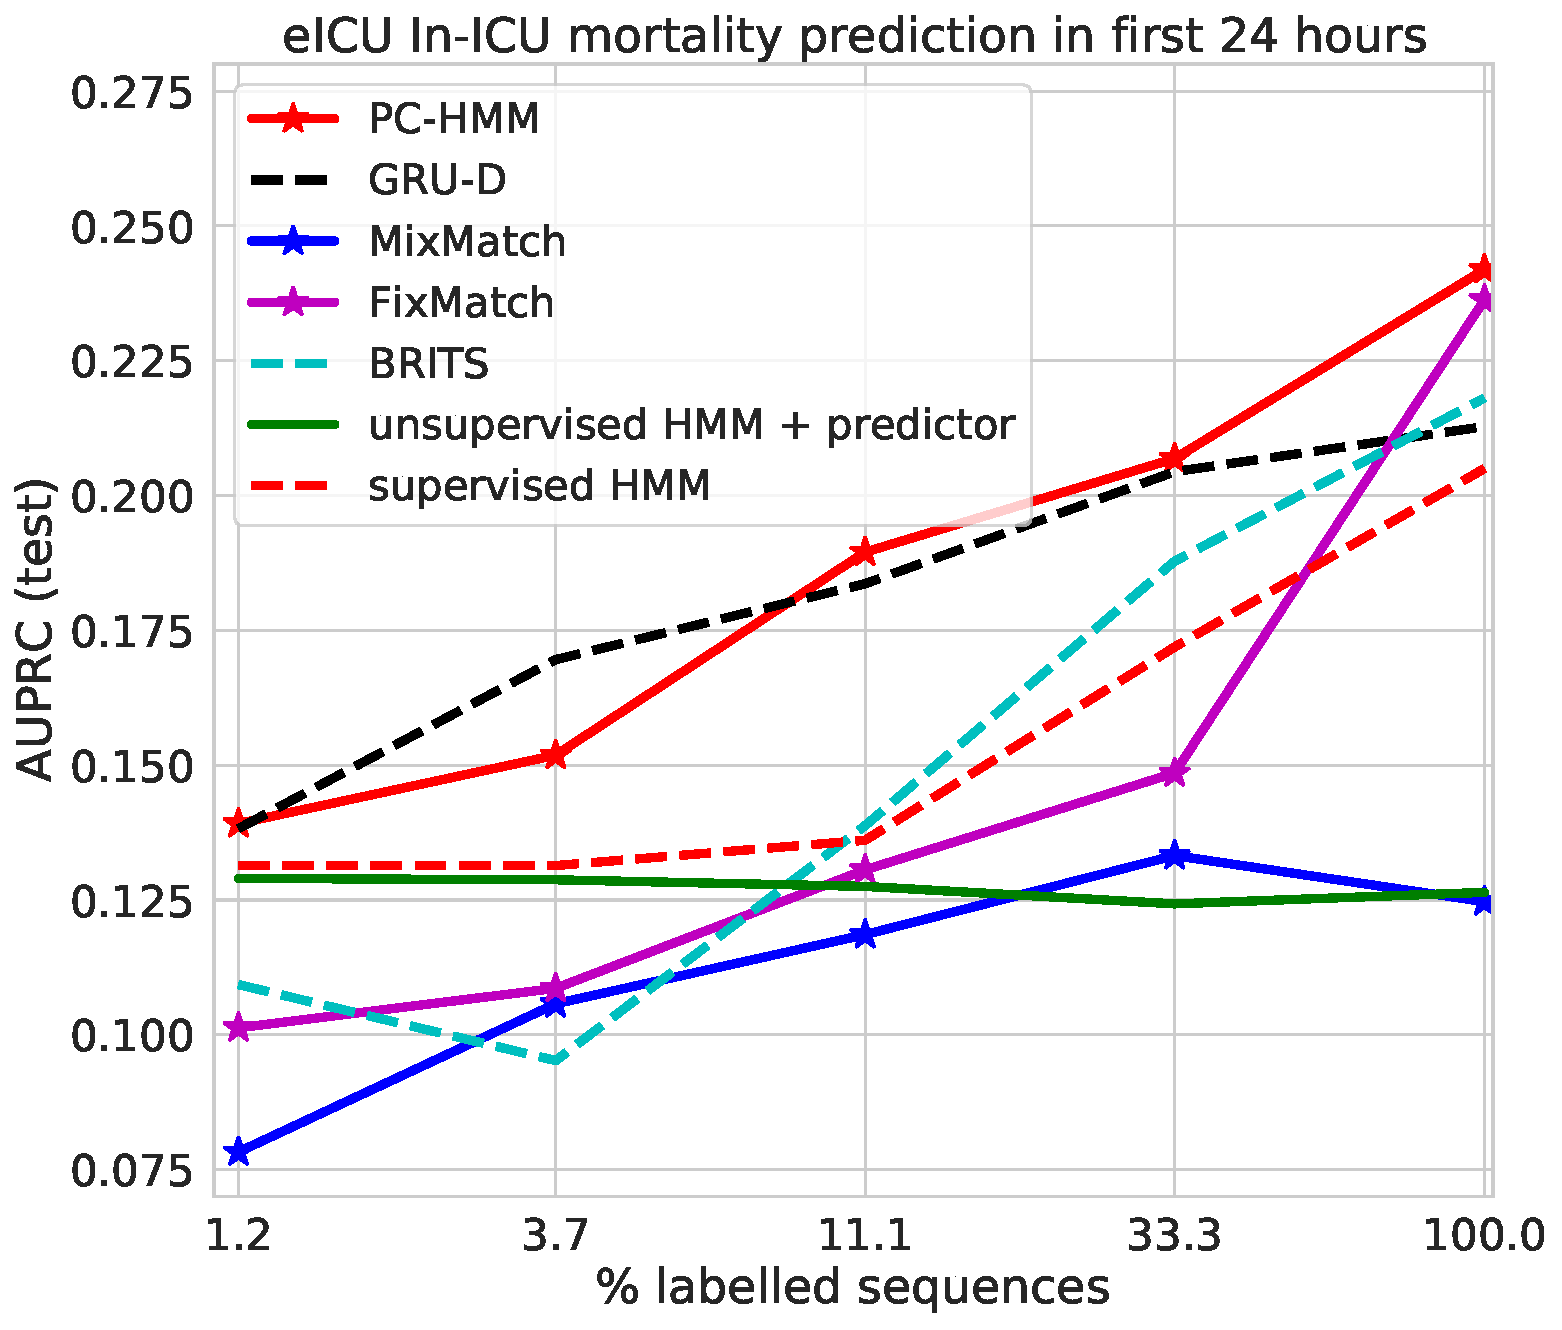
\includegraphics[width=0.5\textwidth]{content/chapters/semi_supervised_pchmm_missing_data/images/perf_mortality_prediction_eicu.pdf}
	&
	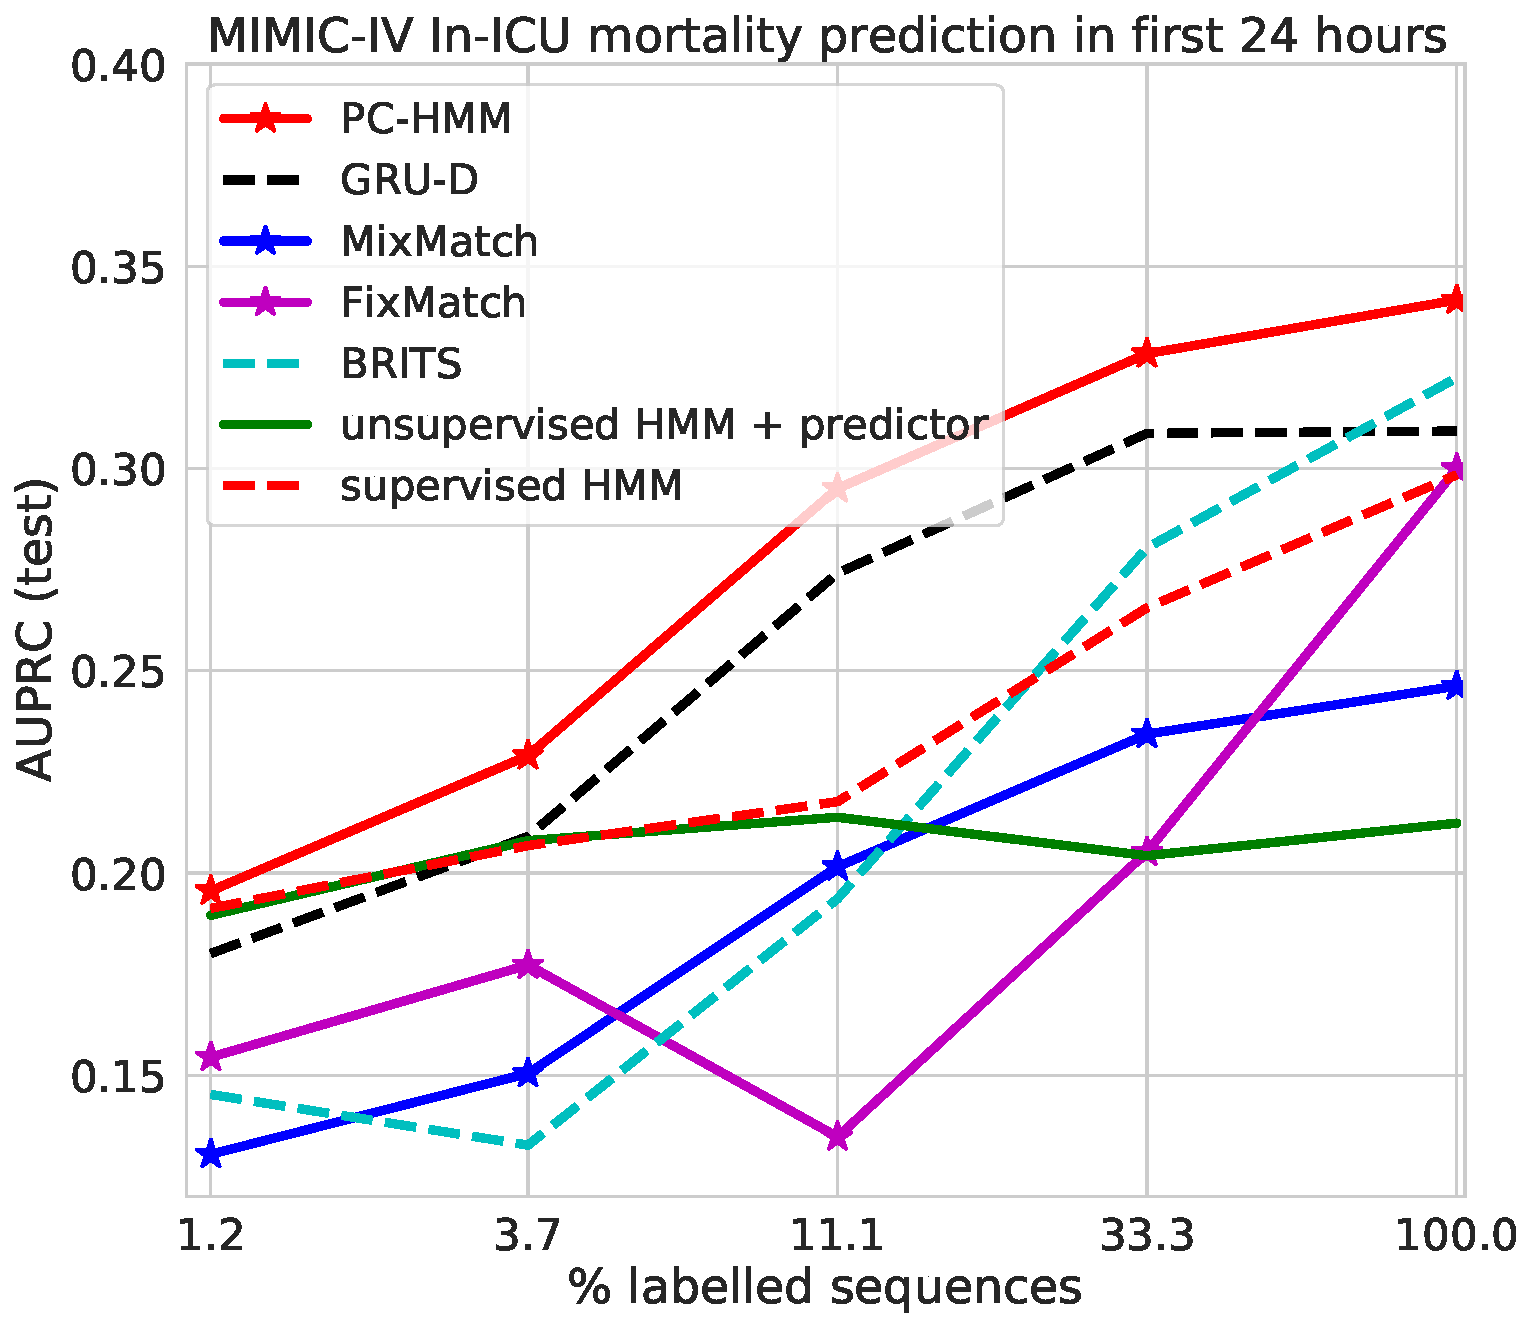
\includegraphics[width=0.5\textwidth]{content/chapters/semi_supervised_pchmm_missing_data/images/perf_mortality_prediction_mimic.pdf}	
\end{tabular}
\caption[AUPRC versus amount of labeled data for in-hospital
mortality early warning classifiers on two large EHR datasets]{AUPRC (higher is better) versus amount of labeled data for in-hospital mortality early warning classifiers on two large EHR datasets (left: eICU, right: MIMIC-IV).
X-axis: Percentage of all training sequences available with labels (SSL methods treat remaining sequences as unlabeled; other methods discard them).
Y-axis: Area under precision-recall curve (AUPRC, higher is better).
%Each line represents a different model.
SSL methods, including our PC-HMM as well as MixMatch and FixMatch,
learn from both labeled and unlabeled data.
GRU-D, BRITS, and Random Forest use the labeled set only.
The PC-HMM matches or beats the other models across all tested labeled set sizes, despite needing fewer parameters and only $1/10^{th}$ of the training time as the other models. }%endcaption

\label{fig:mortality_prediction_results}
\end{figure*}
\subsection{Mortality Prediction Results}
Fig.~\ref{fig:mortality_prediction_results} shows each method's test-set AUPRC (where $y=1$ means death) as label availability $p$ increases.
Across all tested percentages $p$, the PC-HMM is competitive with deep alternatives, including BRITS and GRU-D as well as deep SSL such as FixMatch and MixMatch on both MIMIC and eICU. Notably, the PC-HMM outperforms the baselines with the fewest parameters (see table \ref{table: n_params}), the least training time (see table \ref{table: training_times}) and the fewest number of jobs for hyperparameter search (see table \ref{table: n_params}). The full list of hyperparameters are listed in table \ref{table: hyperparameters}

\begin{table*}[!h]
\begin{tabular}{|l|l|l|l|l|l|l}
\hline
         & \multicolumn{5}{l|}{Confidence Intervals for AUPRC for mortality prediction (100\% labelled)}                                  \\ 
         \hline
         & PC-HMM & GRU-D & MixMatch & FixMatch & BRITS \\ 
         \hline
MIMIC-IV & 0.341 (\scriptsize{0.332, 0.351}) & 0.306 (\scriptsize{0.301, 0.315}) & 0.212 (\scriptsize{0.207, 0.218}) & 0.180 (\scriptsize{0.177, 0.189}) & 0.322 (\scriptsize{0.320, 0.325})  \\ 
\hline
eICU    & 0.243 (\scriptsize{0.239, 0.251}) & 0.211 (\scriptsize{0.209, 0.214}) &  0.126 (\scriptsize{0.120, 0.129})&  0.124 (\scriptsize{0.122, 0.129})&  0.218 (\scriptsize{0.213, 0.220}) \\ 
\hline
\end{tabular}
  \caption[AUPRC with confidence intervals for mortality prediction with all labels known]{AUPRC with confidence intervals for mortality prediction with all labels known. The confidence intervals are obtained by bootstrapping on the test set. We resample 10 different subsets of the test set, and compute AUPRC for each subset. The median (5th, 95th) of the AUPRC across subsets are shown in the table. We find that the variance in prediction across subsets is fairly low and thus only show the performance on the full test set in figures \ref{fig:mortality_prediction_results} and \ref{fig:MIMIC_los_prediction_results}}
    \label{table: CI_performance}
\end{table*}

\begin{table*}[!h]
\begin{tabular}{|l|l|l|l|l|l|}
\hline
Beliefs aggregation  & \multicolumn{5}{l|} {AUPRC for MIMIC-IV mortality prediction varying $p$($\%$ labeled sequences)}\\
\hline
         & $p=1.2$\%      & $p=3.7\%$      & $p=11.1\%$      & $p=33.3\%$      & $p=100\%$     \\
\hline
Average     & 0.19 (\scriptsize{0.18, 0.20})       & 0.23 (\scriptsize{0.22, 0.23})      & 0.29  (\scriptsize{0.29, 0.30})        & 0.32 (\scriptsize{0.32, 0.34})        & 0.34 (\scriptsize{0.33, 0.35})      \\
\hline
1 Conv layer + Max & 0.14 (\scriptsize{0.13, 0.14})       & 0.19 (\scriptsize{0.19, 0.20})      & 0.27  (\scriptsize{0.26, 0.28})        & 0.27 (\scriptsize{0.27, 0.28})        & 0.28 (\scriptsize{0.27, 0.29}) \\
\hline
First + Last Step concat & 0.15 (\scriptsize{0.15, 0.16})       & 0.19 (\scriptsize{0.18, 0.19})      & 0.20  (\scriptsize{0.20, 0.21})        & 0.21 (\scriptsize{0.21, 0.22})        & 0.25 (\scriptsize{0.24, 0.25}) \\
\hline
\end{tabular}
  \caption[Comparison of aggregation strategies of the HMM beliefs, before be-
ing passed as features to the predictor]{Comparison of aggregation strategies of the HMM beliefs, before being passed as features to the predictor. We compare 3 stategies : (1)averaging beliefs across time (2) convolutional transformation of the belief sequence followed by max-pooling \citep{hopePredictionConstrainedHiddenMarkov2021} and (3)concatenating the beliefs at the first and last time steps. Across all levels of missing labels, we observe that averaging the beliefs performs best \citep{sotoodeh2019improving}.}
    \label{table: avg_vs_max_pooling}
\end{table*}

\begin{figure}[!t]
\begin{tabular}{c c}
    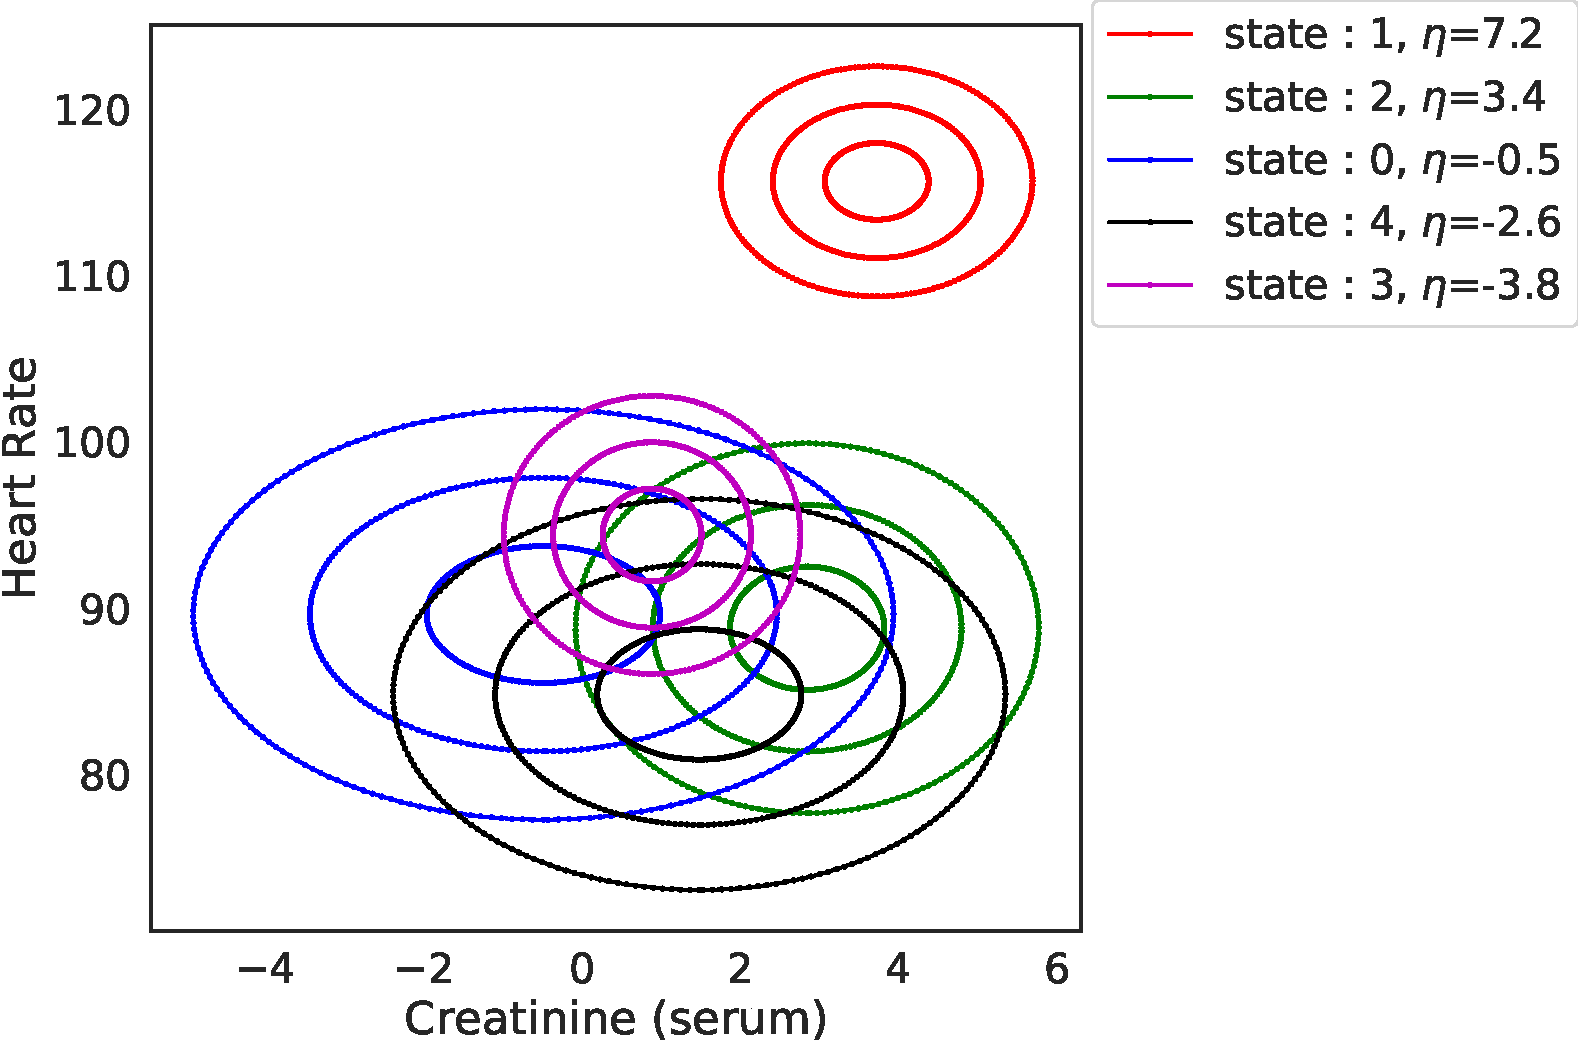
\includegraphics[width=0.5\textwidth]{content/chapters/semi_supervised_pchmm_missing_data/images/interpretability_Heart Rate_Creatinine (serum)_MIMIC.pdf} 
    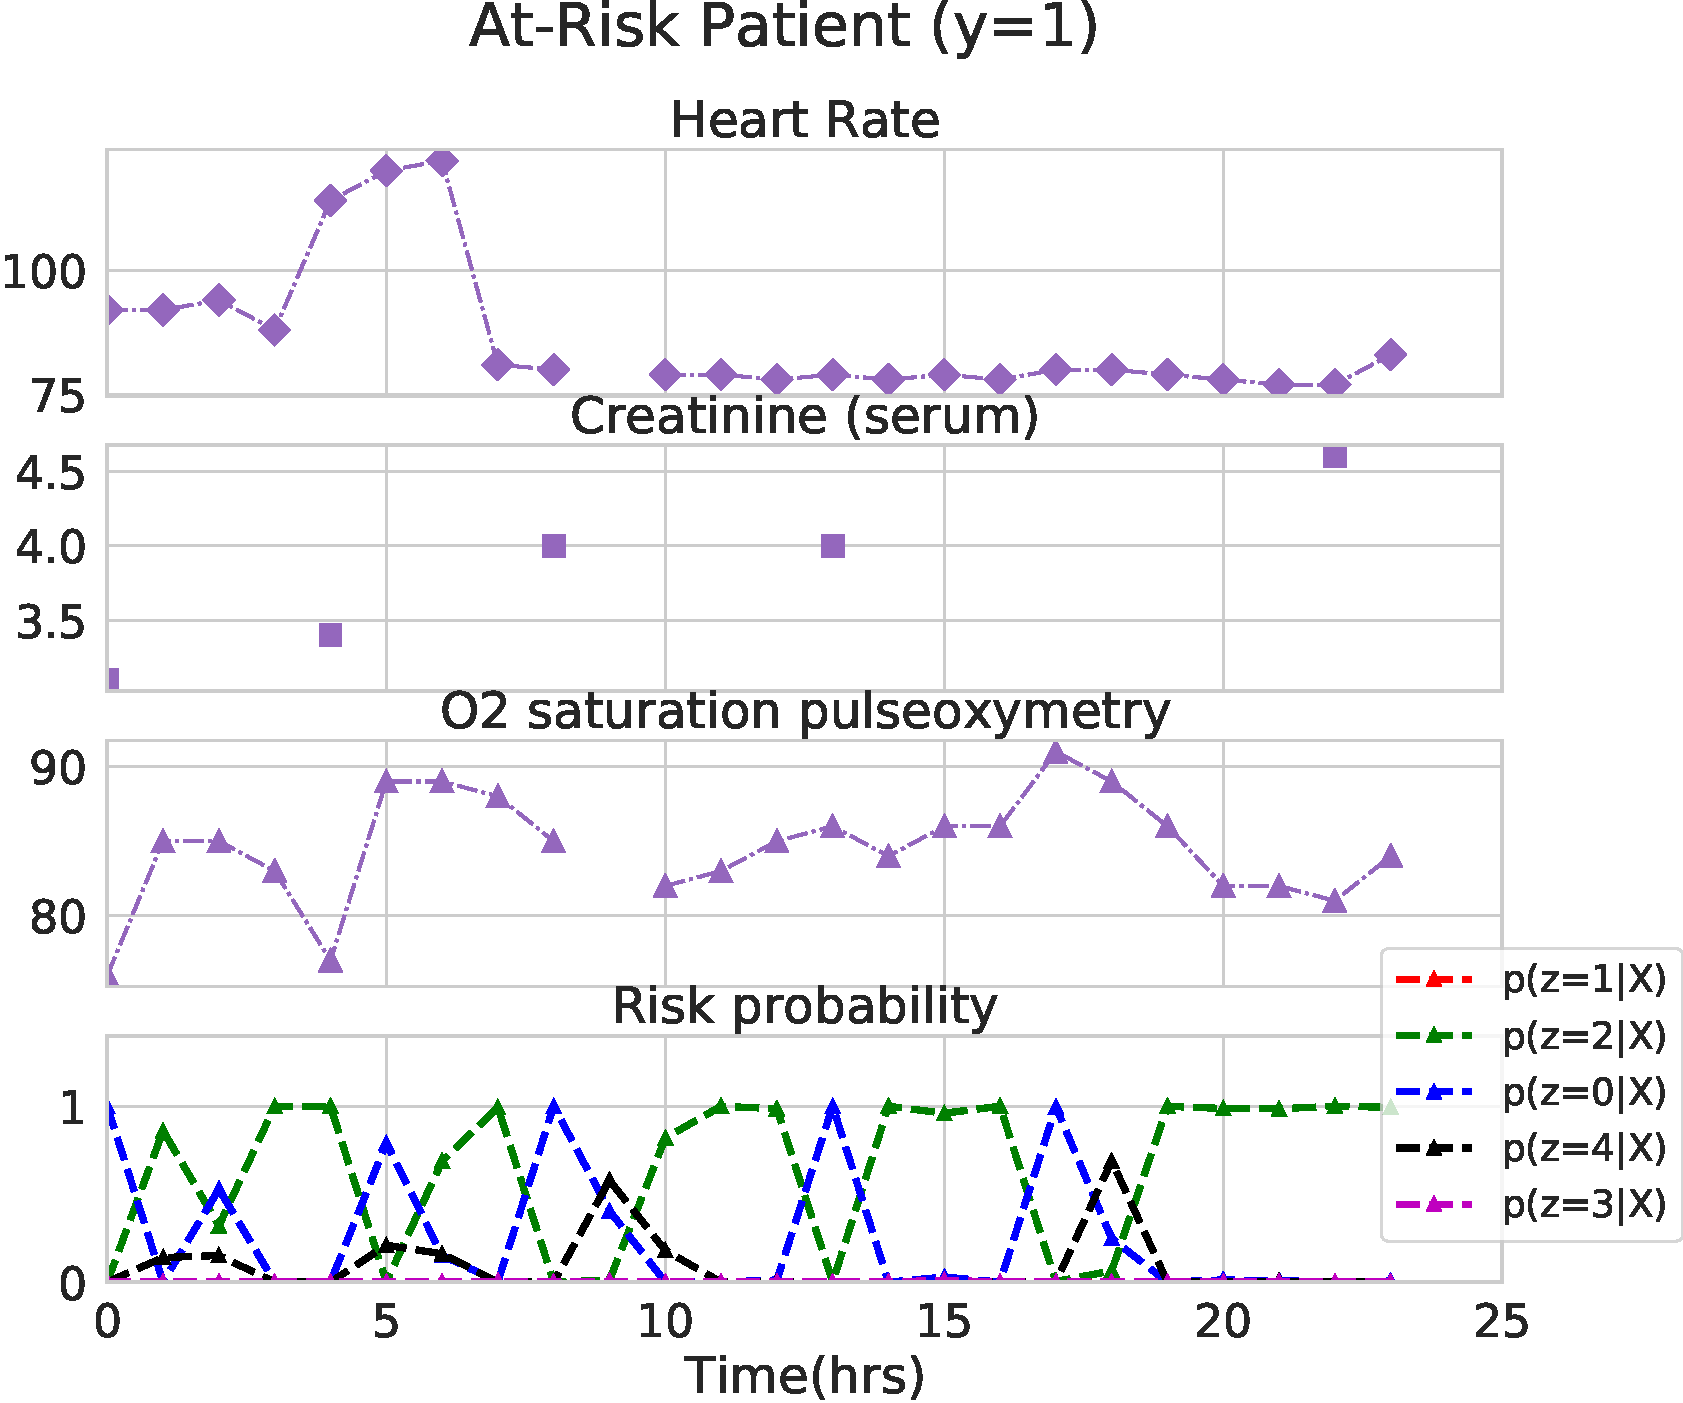
\includegraphics[width=0.5\textwidth]{content/chapters/semi_supervised_pchmm_missing_data/images/mortality_risk_patient_interpretability.pdf} \\
    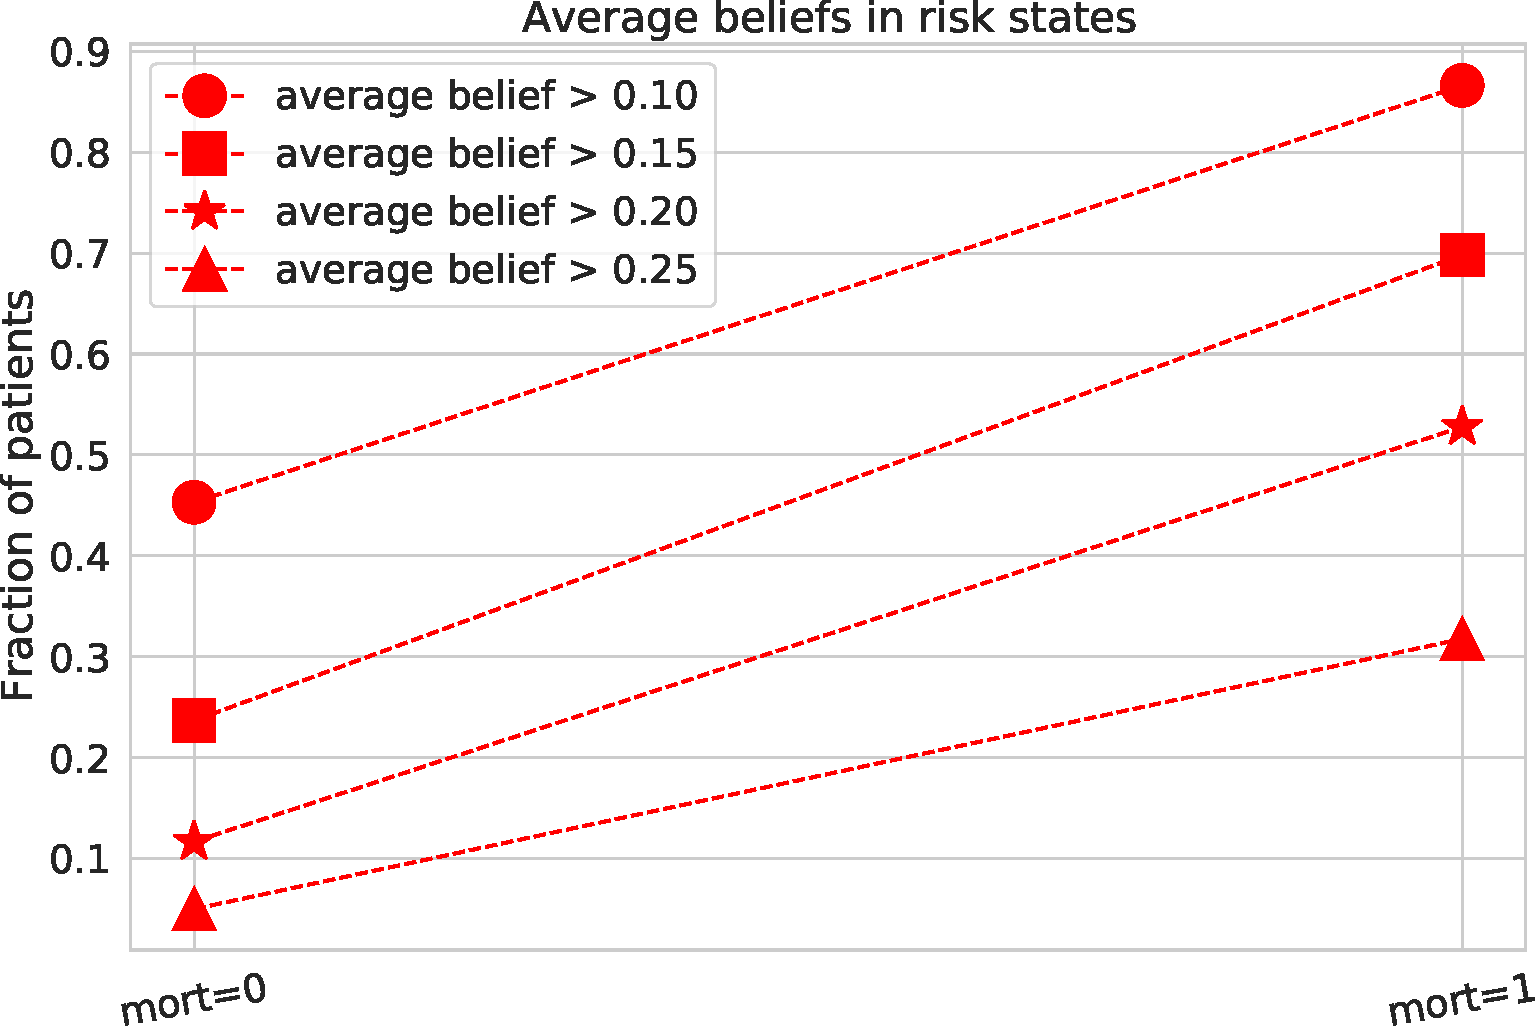
\includegraphics[width=0.5\textwidth]{content/chapters/semi_supervised_pchmm_missing_data/images/avg_beliefs_plots_for_mortality.pdf}
\end{tabular}
\caption[Interpretation of learned PC-HMM for mortality prediction]{
Interpretation of learned PC-HMM on eICU data.
\textbf{\textit{Top Left}}: Gaussian emission distributions of states and their $\eta_k$ (predictor weights).
The red and green states represent high risk (high $\eta_k$).
High risk states seem to represent populations with high heart rate and high creatinine levels (above 1.9mg/dL), which could indicate kidney problems~\citep{baha2021effect}.
\textbf{\textit{Top Right}}: For a patient labeled $y=1$ (who eventually dies), high heart rate and high creatinine are observed throughout the stay, and thus beliefs $b_t$ give highest probability to high risk states.
The probability of state $2$ (green) peak during segments of high creatinine and low oxygen saturation
\textbf{\textit{Bottom}}: We show the average beliefs (averaged over time) of normal patients and risk patients. Clearly, patients at risk spend more time in the risk state compared to the normal patients.
}%endcaption
\label{fig:interpretability_mortality}
\end{figure}

\begin{figure}[!ht]
\begin{center}
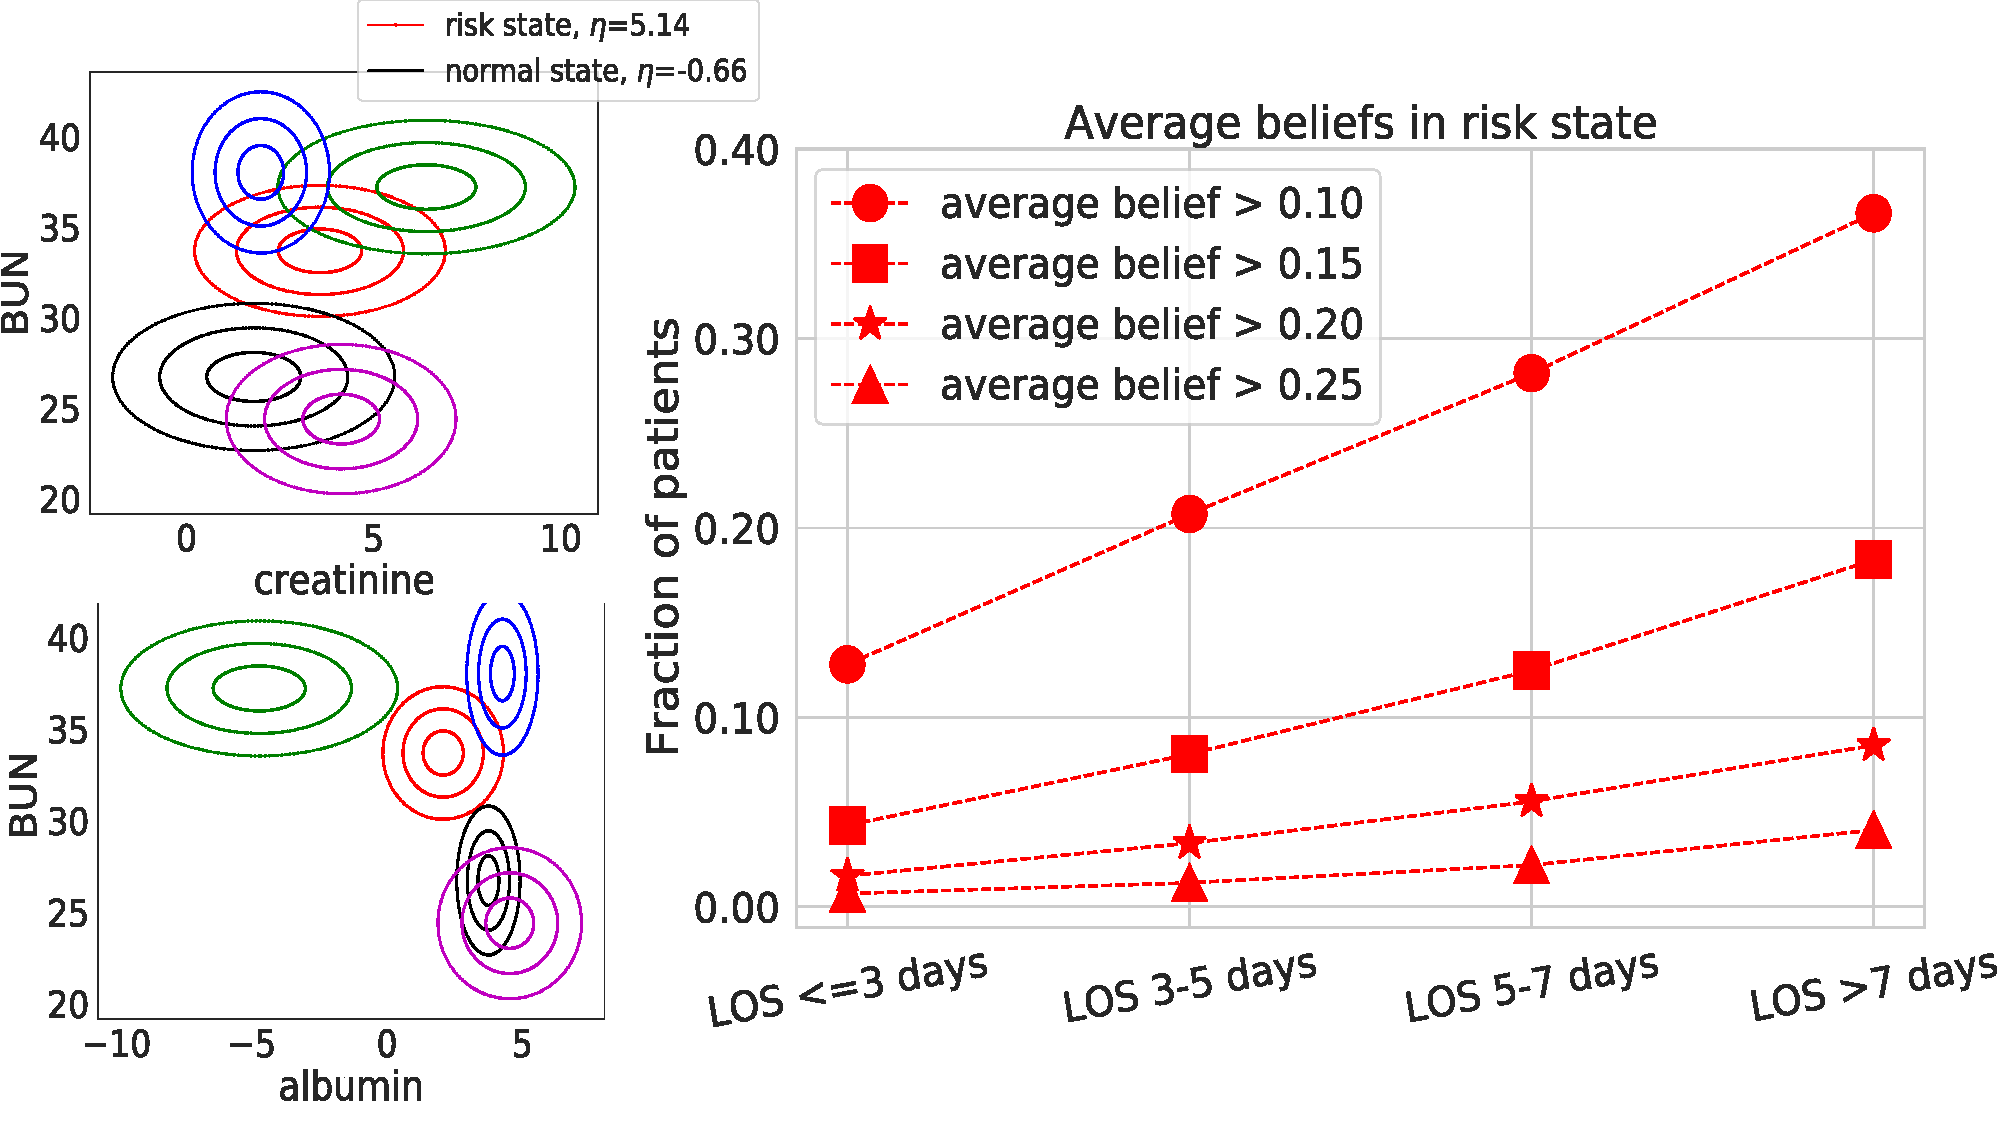
\includegraphics[width=1.0\textwidth]{content/chapters/semi_supervised_pchmm_missing_data/images/interpretability_plot_eicu_2.pdf}
\caption[Interpretability of learned PC-HMM for Length of stay prediction]{\textbf{Left} : Our PC-HMM model reveals five states, representing different risk levels. The red state indicates the `risk state' associated with high BUN and low albumin and high creatinine. \textbf{Right}: We show the average beliefs, averaged over time, in the `risk state'. Notably, as the LOS increases, the average beliefs in the `risk state' increases. 
}%endcaption
\label{fig:interpretability_los_prediction}
\end{center}
\end{figure}

\subsection{Length of Stay Prediction}
Figure \ref{fig:MIMIC_los_prediction_results} plots AUPRC as a function of available labeled data in an SSL setting for MIMIC-IV.
Two major takeaways are apparent.
First, ordinal regression CLMs outperform binary classifiers regardless of whether HMM or neural representations are used.
Second, PC-HMM implementations outperform all other deep learning baselines. Compared to all other baselines, the ordinal regression PC-HMM not only achieves the best performance but also does so with the fewest trainable parameters and lowest training time. 
\begin{figure*}[ht]
\begin{tabular}{@{}c@{\hspace{0.005in}}c@{\hspace{0.005in}}c@{}}
	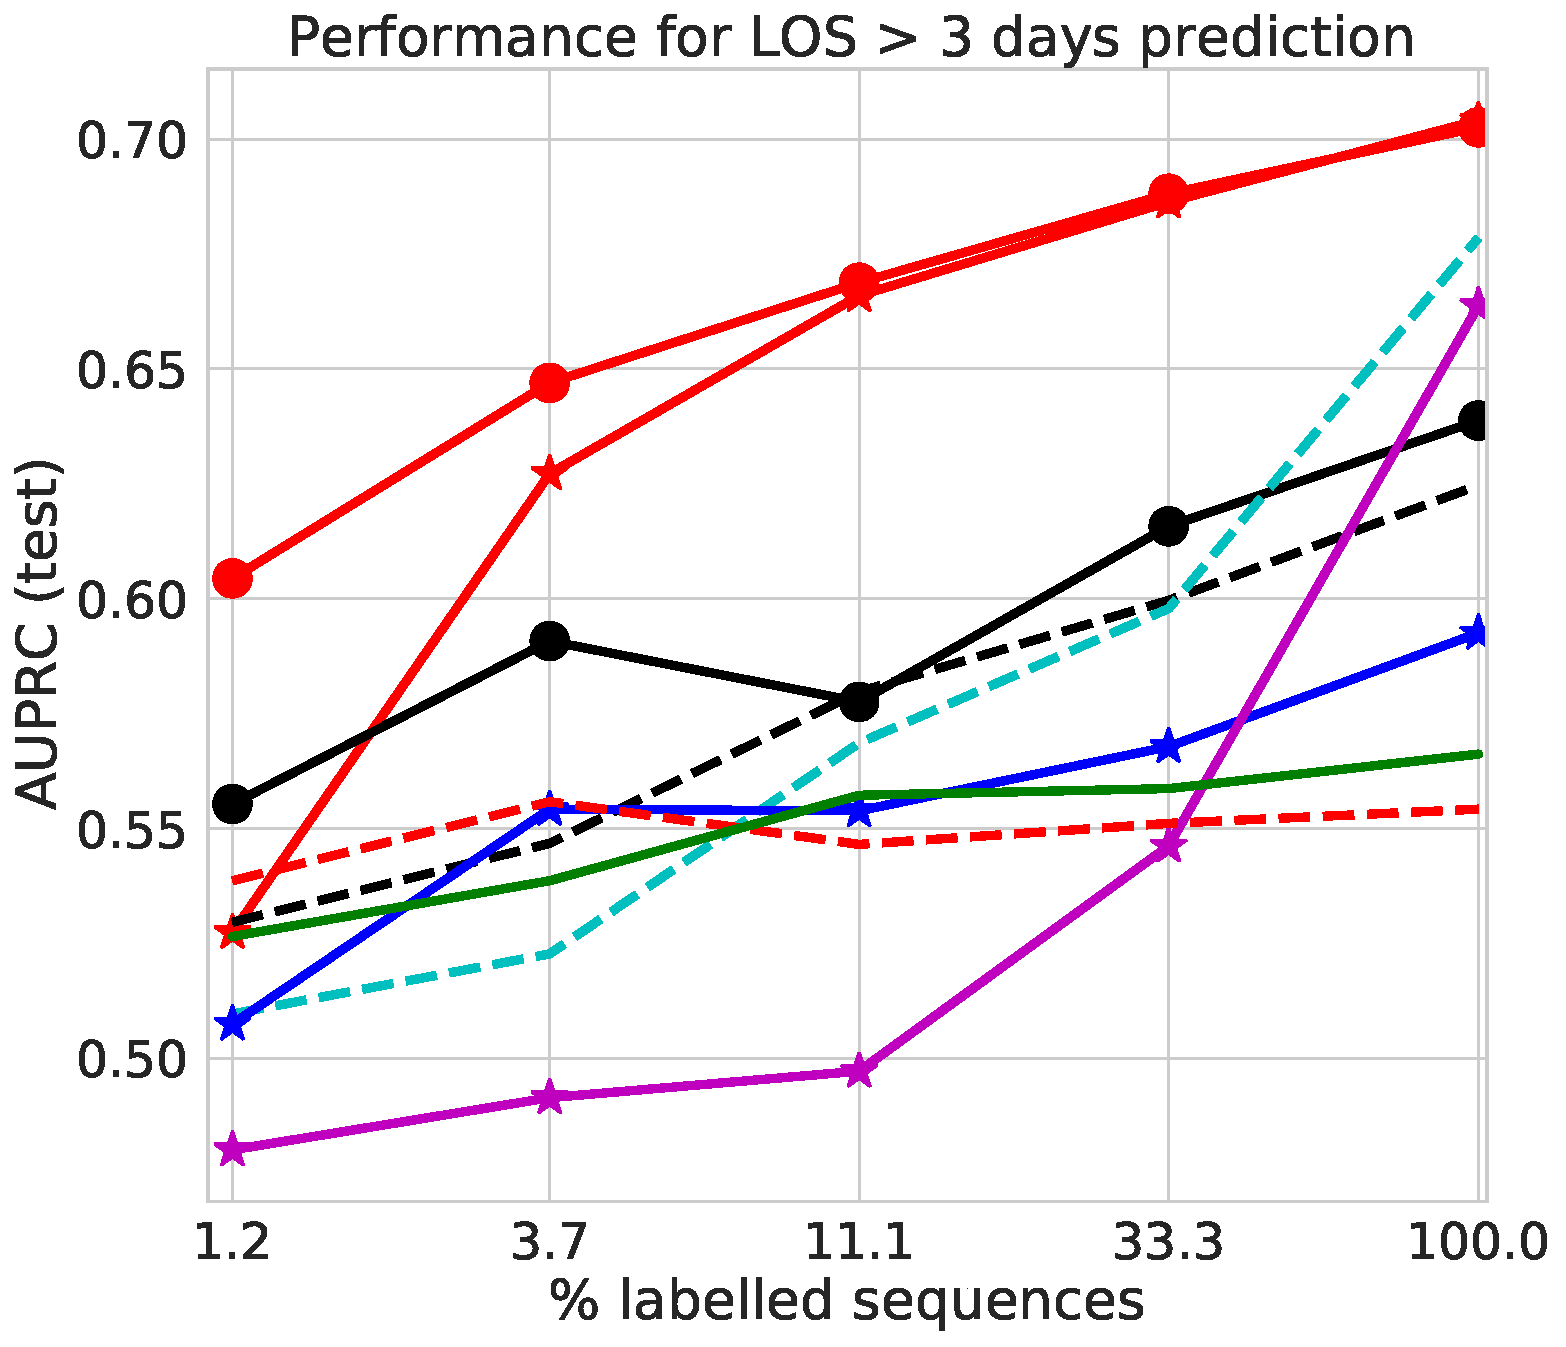
\includegraphics[width=0.35\textwidth]{content/chapters/semi_supervised_pchmm_missing_data/images/perf_los_geq_3_days.pdf}
	&
	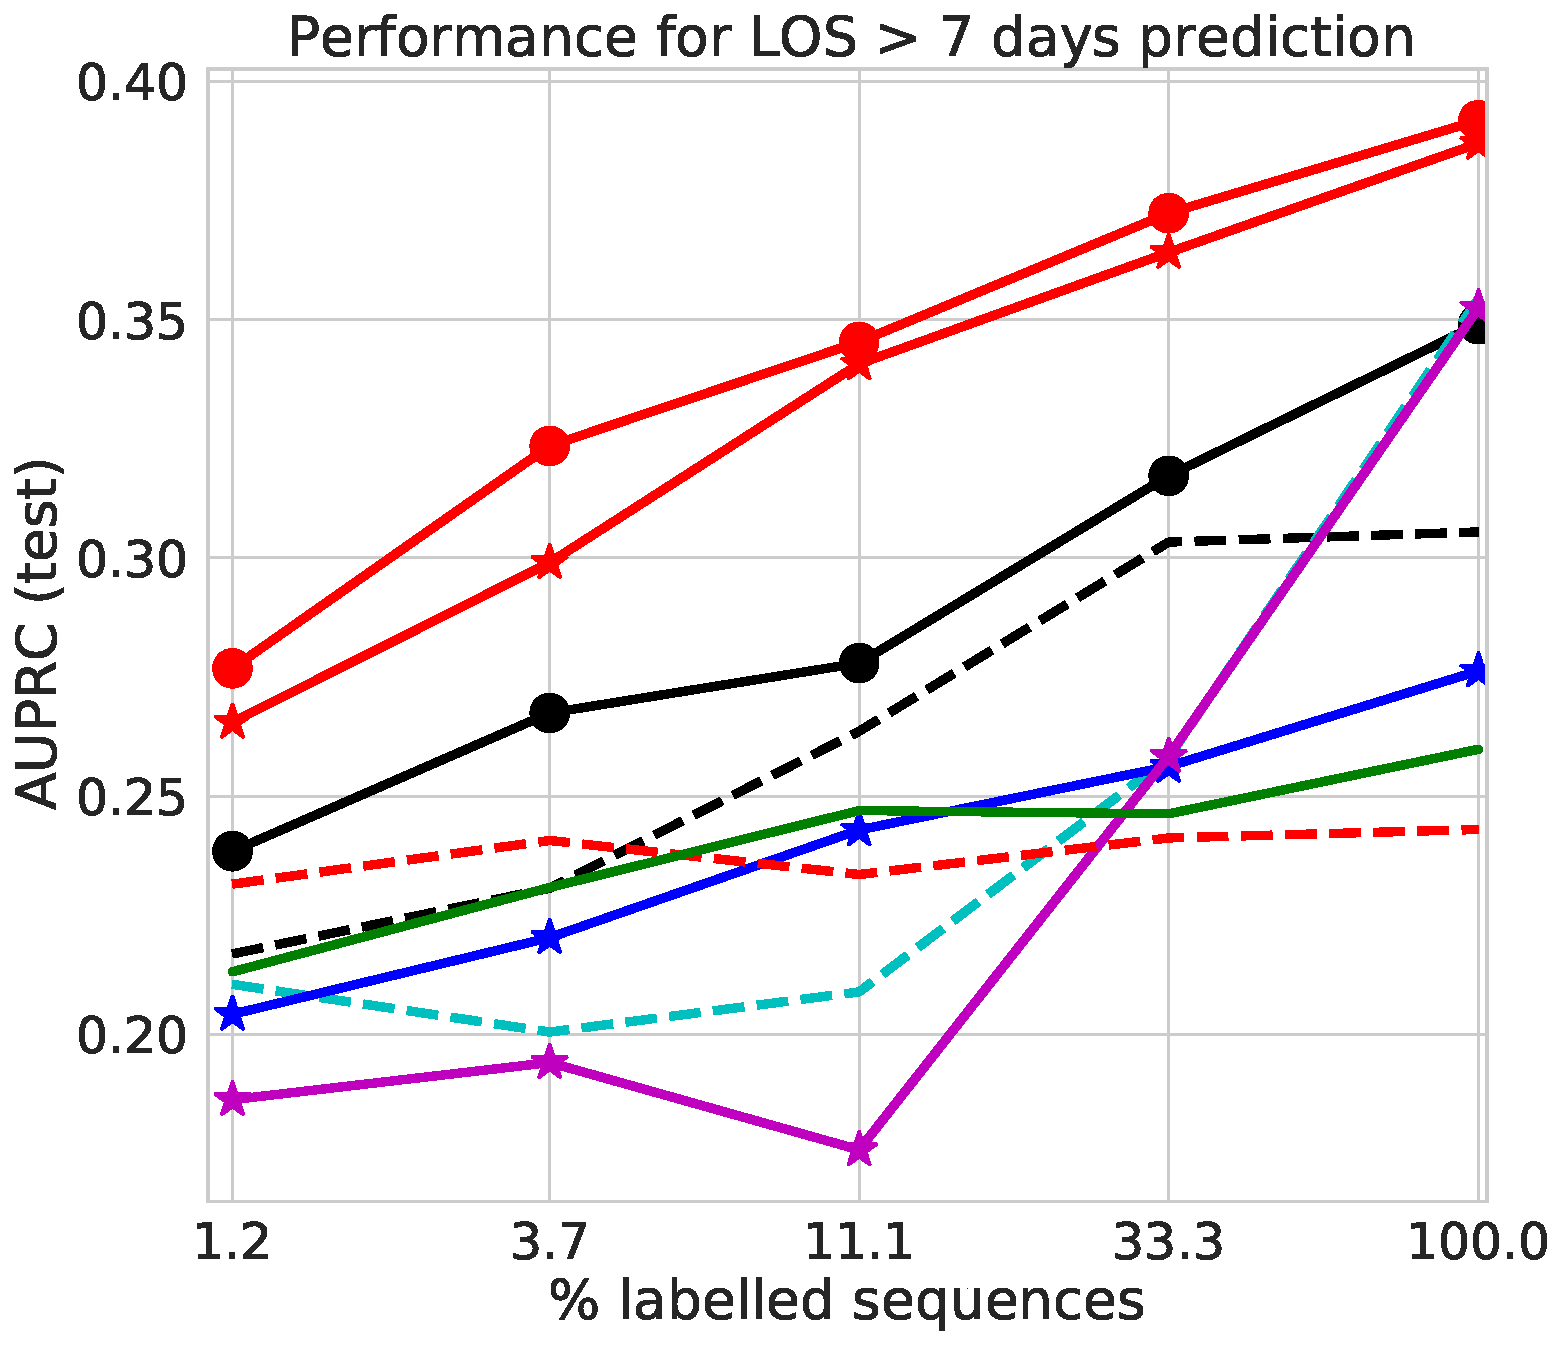
\includegraphics[width=0.35\textwidth]{content/chapters/semi_supervised_pchmm_missing_data/images/perf_los_geq_7_days.pdf}	
 	&
	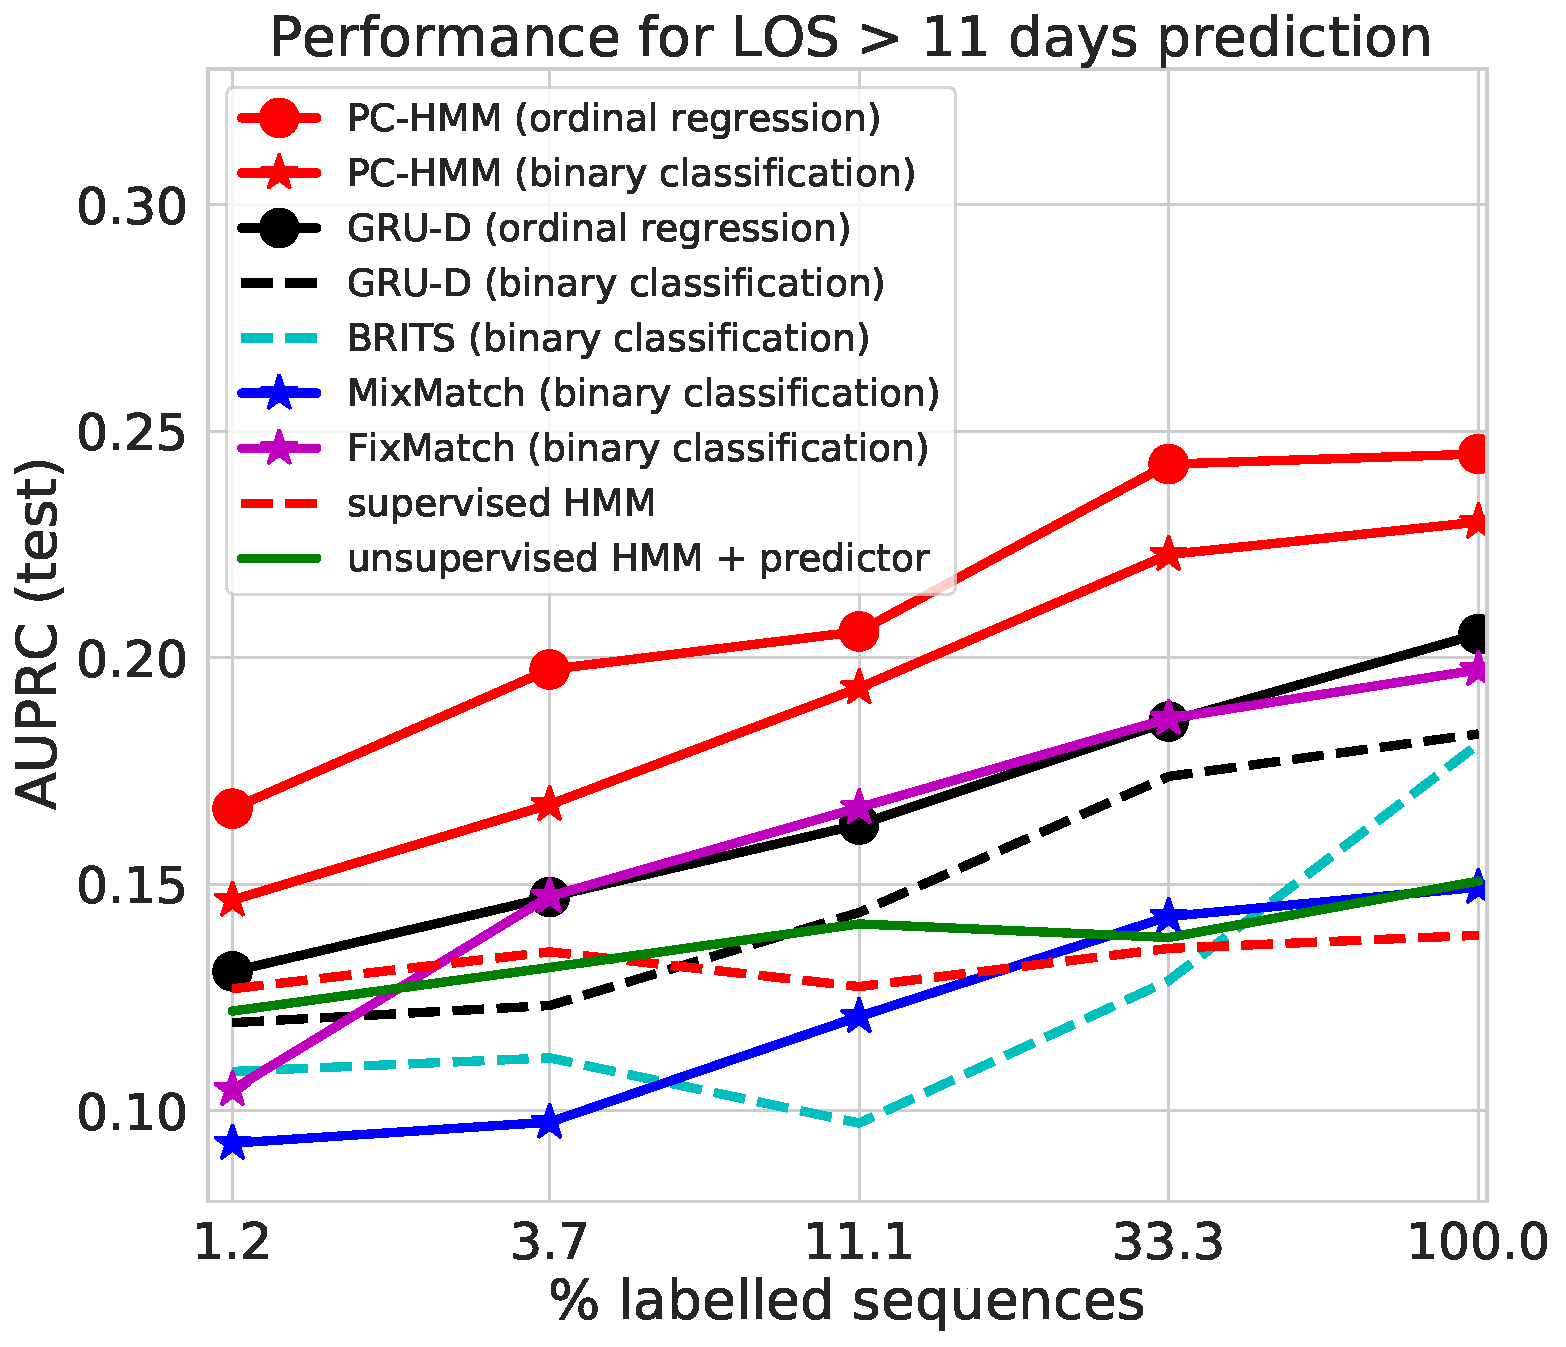
\includegraphics[width=0.35\textwidth]{content/chapters/semi_supervised_pchmm_missing_data/images/perf_los_geq_11_days.pdf}	
\end{tabular}
\caption[AUPRC versus amount of labeled data for length-of-stay prediction on MIMIC-IV at 3 ordinal labels ($>3$, $>7$, and $>11$ days)]{AUPRC (higher is better) versus amount of labeled data for length-of-stay prediction on MIMIC-IV at 3 ordinal labels ($>3$, $>7$, and $>11$ days).
SSL methods (PC-HMM, MixMatch, and FixMatch)
learn from both labeled and unlabeled data.
GRU-D \citep{cheRecurrentNeuralNetworks2018} and BRITS \citep{caoBRITSBidirectionalRecurrent2018} use the labeled set only.
Binary classification models require 3 separate models (1 for each label), whereas ordinal regression using CLMs require a single model to predict all 3 labels. }%endcaption
\label{fig:MIMIC_los_prediction_results}
\end{figure*}

\input{content/chapters/semi_supervised_pchmm_missing_data/fig_results_eicu_los_prediction}


\subsection{Interpretation of Learned PCHMM States}
Our PC-HMM framework enables us to interpret cohorts of vulnerable populations by visualizing the emission distributions for the states that have the highest predictor coefficients $\eta_k$.
% Some of these cohorts from eICU are visualized in Figure \ref{fig:interpretability}. 
On eICU data, Fig.~\ref{fig:interpretability_mortality} shows our PC-HMM identifies states representing high blood urea nitrogen (BUN) and high creatinine (common indicators of kidney failure \citep{baha2021effect}) as the most vulnerable to in-ICU mortality. 
The model transitions to these `high-risk' states as soon as high values of creatinine and BUN are observed in a patient who eventually dies.
Additionally, we illustrate the interpretability of the PC-HMM trained to predict length of stay in Figure \ref{fig:interpretability_los_prediction}, highlighting that longer stays are associated with larger beliefs in the `risk state'.


\subsection{Training times for each model}
\begin{table}[H]
\centering
\begin{tabular}{|l|l|l|l|l|l|l|}
\hline
 & & \multicolumn{5}{l|}{\textit{seconds/epoch} to train each model} \\
\hline
    Dataset & & PC-HMM & GRU-D & MixMatch      & FixMatch      & BRITS     \\
\hline
MIMIC-IV & $D=41$ features & 9   & 43       & 70         & 55         &  48     \\
\hline
eICU    & $D=41$ features & 16        & 70       & 115         & 90   &  75     \\
\hline
\end{tabular}
  \caption[Computation time (seconds/epoch) required per model]{Computation time (seconds/epoch) required by each model. An epoch is completed when every example in the training set is covered at-least once. Although computation time increases when measurements are more frequent, the PC-HMM still requires far lesser time to train due to significantly lesser parameters than the other models.}
    \label{table: training_times}
\end{table}

\subsection{Parameter counts and Hyperparameter search for each model}
\begin{table}[H]
\centering
\begin{tabular}{|l|l|l|l|l|l|}
\hline
     & PC-HMM & GRU-D & MixMatch  & FixMatch      & BRITS     \\
\hline
Parameters & 452-2,102  & 12,739-87,523   & 2,866-45,634  & 2,866-45,634  &  48,850-252,370     \\
\hline
Jobs & 900 & 7,560 & 10,800 & 21,600 &  6,480     \\
\hline
Training time(per job) & 1-2 hrs & 5-6 hrs & 6-8 hrs & 4-6 hrs &  4-5 hrs  \\
\hline
\end{tabular}
  \caption[Range of parameter counts and number of jobs for hyperparameter search per model]{Range of parameter counts and number of jobs for hyperparameter search for each model. The PC-HMM requires the fewest parameters, least number of jobs for hyperparameter search, and the least training time and yet produces the best performance.}
    \label{table: n_params}
\end{table}

\newcommand{\tabitem}{~~\llap{\textbullet}~~}
\begin{table*}[!t]
  \centering
  \begin{tabular}{|l|l|l|}
    \hline
    Model & Hyperparameters searched & Selection criterion\\
    \hline
    PC-HMM & \tabitem learning rate : $0.001, 0.01, 0.1$ & Best validation AUPRC  \\
    & \tabitem states : $5, 10, 20$ & \\
    & \tabitem initialization seeds : 5 & \\
    & \tabitem l2 penalty : $0, 0.01, 0.1, 1$ & \\
    & \tabitem $\lambda$ : $50, 100, 500, 1000, 5000$ & \\
    \hline
    GRU-D & \tabitem learning rate : $0.001, 0.01, 0.1$ & Best validation AUPRC \\
    & \tabitem hidden units : $32, 64, 128$ & with early stopping \\
    & \tabitem hidden layers : $1, 2$ & \\
    & \tabitem initialization seeds : 20 & \\
    & \tabitem l2 penalty : 7 log-spaced values between $10^-6$ and $100$ & \\
    & \tabitem batch-size : $128, 256, 512$ & \\
    \hline
    BRITS & \tabitem learning rate : $0.001, 0.01, 0.1$ & Best validation AUPRC\\
    & \tabitem hidden units : $32, 64, 128$ & with early stopping \\
    & \tabitem initialization seeds : 20 & \\
     & \tabitem hidden layers : $1, 2$ & \\
    & \tabitem dropout : $0, 0.1, 0.25$ & \\
    & \tabitem batch-size : $128, 256, 512$ & \\
    & \tabitem imputation-weight : $0.3, 0.6$ & \\
    & \tabitem label weight : $1.0$ & \\
    \hline
    FixMatch & \tabitem learning rate : $0.001, 0.01, 0.1$ & Best validation AUPRC \\
    & \tabitem hidden units : 16, 32, 64 & with early stopping \\
    & \tabitem initialization seeds : 5 & \\
    & \tabitem hidden layers : $1, 2$ & \\
    & \tabitem batch-size : $128, 256, 512$ & \\
    & \tabitem l2 penalty : 5 log-spaced values between $10^-8$ and $10$ & \\
    & \tabitem pseudo-label thresholds : $0.6, 0.8$ & \\
    & \tabitem augmentation noise variance : $0.1, 0.01$ & \\
    & \tabitem unlabeled strength : $50, 75$ & \\
    & \tabitem Temperature scaling : $0.5$ & \\
    & \tabitem $\alpha$(for MixUp): $0.75$ & \\
    \hline
    MixMatch & Same hyperparameter grid as FixMatch & Best validation AUPRC \\
    & except no psuedo-label thresholds & with early stopping\\
    % \hline
    % Random Forest & \tabitem Fraction of  features : $0.33, 0.66, 1.0$ & Best validation AUPRC \\
    % & \tabitem Max leaf nodes : 32, 64, 128 & \\
    % & \tabitem Min Samples per leaf : 64, 128, 512, 1024 & \\
    % & \tabitem Estimators : 64 & \\
    \hline
  \end{tabular}
  \caption{Hyperparameters for all the models}
  \label{table: hyperparameters}
\end{table*}